
\chapter[Lý thuyết: Công suất tiêu thụ của\\ mạch điện xoay chiều. Hệ số công suất;\\Dạng bài: Xác định công suất tiêu thụ của mạch điện xoay chiều]{Lý thuyết: Công suất tiêu thụ của mạch điện xoay chiều. Hệ số công suất;\\Dạng bài: Xác định công suất tiêu thụ của mạch điện xoay chiều}
\section{Lý thuyết}

\subsection{Công suất của mạch điện xoaychiều}
\subsubsection{Biểu thức của công suất}
$$\calP =UI\cos\varphi ,$$
trong đó:
\begin{itemize}
	\item $U$ là \bltext{điện áp hiệu dụng} $\left( \si{\volt} \right)$;
	\item $I$ là \bltext{cường độ dòng điện hiệu dụng} $\left(\textrm{A} \right)$;
	\item $\varphi$ là \bltext{độ lệch pha} giữa $u$ và $i$ $\left( \textrm{rad} \right)$;
	\item $\calP$ là \bltext{công suất} $\left( \si{\watt} \right)$.
\end{itemize}
\subsubsection{Điện năng tiêu thụ của mạch điện}
$$W =\calP t ,$$
trong đó:
\begin{itemize}
	\item $\calP$ là \bltext{công suất tiêu thụ} của mạch điện $\left( \si{\watt} \right)$;
	\item $t$ là \bltext{thời gian dòng điện qua mạch} $\left(\textrm{s} \right)$;
	\item $W$ là \bltext{điện năng tiêu thụ} của mạch điện.
\end{itemize}
\subsection{Hệ số công suất}
Trong công thức tính công suất, $\cos \varphi$ gọi là \bltext{hệ số công suất} có giá trị \bltext{$0\leq \cos \varphi \leq 1.$}
$$\cos\varphi =\dfrac{U_R}{U}\qquad\textrm{hay}\quad \cos \varphi =\dfrac{R}{Z},$$
trong đó:
\begin{itemize}
	\item $U_R$, $U$ lần lượt là điện áp hiệu dụng giữa hai đầu điện trở và điện áp hiệu dụng giữa hai đầu đoạn mạch;
	\item $R$ là điện trở và $Z$ là tổng trở. 
\end{itemize}	
\subsection{Các công thức thường sử dụng}
\begin{itemize}
	\item  Công thức tính công suất của mạch điện xoay chiều $R, L, C$ mắc nối tiếp:
	\begin{equation*}
		\calP=UI\cos \varphi=UI\cos (\varphi_u-\varphi_i),
	\end{equation*}
	\begin{equation*}
		\calP=I^2R=\dfrac{U^2}{Z^2}R=\dfrac{U^2}{R} \cos^2 \varphi.
	\end{equation*}
	\item Mạch điện không có $R$ thì $\calP=0$.
	\item Mạch điện $R, L, C$ cộng hưởng thì $\calP=UI=\dfrac{U^2}{R}=I^2R$.
\end{itemize}

\subsection{Phương pháp giải chung}

\begin{description}
	\item[Bước 1] Xác định mạch điện xoay chiều đó gồm những phần tử nào trong $R$, $L$, $r$, $C$. 
	\item [Bước 2] Áp dụng công thức 
	\begin{equation*}
		I=\dfrac{I_0}{\sqrt 2}; U=\dfrac{U_0}{\sqrt 2}
	\end{equation*}
	để tìm $U$ và $I$.
	\item[Bước 3] Xác định hệ số công suất $\cos \varphi =  \dfrac{R}{Z}$ hoặc $\varphi = \varphi_u -\varphi_i$.
\end{description}


\section{Mục tiêu bài học - Ví dụ minh họa}

\begin{dang}{Ghi nhớ được công thức tính\\ công suất điện, hệ số công suất}
	\viduii{2}{Đặt điện áp xoay chiều vào hai đầu đoạn mạch có $R$, $L$, $C$ mắc nối tiếp. Hệ số công suất của đoạn mạch \textbf{không} phụ thuộc vào
		\begin{mcq}
			\item tần số của điện áp đặt vào hai đầu đoạn mạch.
			\item điện trở thuần của đoạn mạch.
			\item điện áp hiệu dụng đặt vào hai đầu đoạn mạch.
			\item độ tự cảm và điện dung của đoạn mạch.
		\end{mcq}
	}
	{	\begin{center}
			\textbf{Hướng dẫn giải}
		\end{center}
		
		Ta có hệ số công suất của đoạn mạch được xác định bởi công thức:
		$$\cos \varphi = \dfrac{R}{Z} = \dfrac{R}{\sqrt{R^2 + \left(\omega L - \dfrac{1}{\omega C}\right)^2}}.$$
		
		Hệ số công suất phụ thuộc vào $R$, $L, C, f$ và không phụ thuộc vào $U$.
		
		\textbf{Đáp án: C}.
	}
	\viduii{3}{Đặt vào 2 đầu đoạn mạch gồm $R, L, C$ mắc nối tiếp một điện áp xoay chiều $u = U_0\cos \omega t\ \text{V}$ thì cường độ dòng điện trong mạch có biểu thức $i = I_0\sin \left(\omega t + \dfrac{\pi}{6}\right)\ \text{A}$. Công suất điện tiêu thụ của đoạn mạch là
		\begin{mcq}(4)
			\item $\dfrac{U_0I_0}{2}$.
			\item $\dfrac{U_0I_0\sqrt 3}{4}$.
			\item $\dfrac{U_0I_0}{4}$.
			\item $\dfrac{U_0I_0\sqrt 3}{2}$.
		\end{mcq}
	}
	{	\begin{center}
			\textbf{Hướng dẫn giải}
		\end{center}
		
		Ta có:
		$$i = I_0\sin \left(\omega t + \dfrac{\pi}{6}\right)\ \text{A}.$$
		$$i = I_0 \cos \left(\omega t - \dfrac{\pi}{3}\right)\ \text{A}.$$
		Ta lại có:
		$$\varphi = \varphi_u - \varphi_i= \dfrac{\pi}{3}.$$
		
		Công suất điện tiêu thụ của đoạn mạch là:
		$$\calP = UI\cos \varphi = \dfrac{U_0I_0}{4}.$$
		
		\textbf{Đáp án: C}.
	}
\end{dang}

\begin{dang}{Xác định công suất tiêu thụ toàn mạch}
	\viduii{3}{Đặt điện áp $u={{U}_{0}}\cos \left( \omega t+\dfrac{\pi }{3} \right)~\left( \text{V}\right) $ vào hai đầu đoạn mạch gồm điện trở thuần, cuộn cảm thuần và tụ điện mắc nối tiếp. Biểu thức cường độ dòng điện trong mạch là $i=\sqrt{6}\cos \left( \omega t+\dfrac{\pi }{6} \right)~\left( \text{A}\right) $ và công suất tiêu thụ của đoạn mạch là $150~\text{W}$. Tìm ${{U}_{0}}$.
		\begin{mcq}(4)
			\item $100\sqrt{2}~\text{V}$.
			\item $100~\text{V}$.
			\item $200\sqrt{2}~\text{V}$.
			\item $200~\text{V}$.
		\end{mcq}
	}
	{	\begin{center}
			\textbf{Hướng dẫn giải}
		\end{center}
		
		Cường độ dòng điện hiệu dụng qua mạch: $$I=\dfrac{{{I}_{0}}}{\sqrt{2}}=\sqrt{3}~\text{A}.$$
		
		Độ lệch pha giữa $u$ và $i$: $\varphi ={{\varphi }_{u}}-{{\varphi }_{i}}=\dfrac{\pi }{6}~\text{rad}$.
		
		Hệ số công suất của mạch: $\cos \varphi =\cos \dfrac{\pi }{6}=\dfrac{\sqrt{3}}{2}$.
		
		Ta thay các đại lượng vừa tìm được vào công thức ban đầu:
		
		$$\calP=UI\cos \varphi \Rightarrow U=\dfrac{\calP}{I\cos \varphi }=100~\text{V}.$$
		
		Điện áp cực đại: ${{\text{U}}_{\text{0}}}=\text{U}\sqrt{2}=100\sqrt{2}\text{ }\!\!~\!\!\text{ V}$.
		
		\textbf{Đáp án: A}.
	}
	\viduii{2}{Đặt một điện áp xoay chiều vào hai đầu một mạch điện gồm một điện trở $R = 12\ \Omega$ và một cuộn cảm thuần $L$ mắc nối tiếp. Điện áp hiệu dụng hai đầu đoạn mạch là $\SI{26}{V}$, hai đầu cuộn cảm thuần là $\SI{10}{V}$. Công suất tiêu thụ của đoạn mạch là
		\begin{mcq}(4)
			\item $\SI{12}{W}$.
			\item $\SI{48}{W}$.
			\item $\SI{24}{W}$.
			\item $\SI{16}{W}$.
		\end{mcq}
	}
	{	\begin{center}
			\textbf{Hướng dẫn giải}
		\end{center}
		
		Ta có:
		$$U^2 = U^2_R - U^2_L \Rightarrow U_R = \sqrt {U^2 - U^2_L} = \SI{24}{V}.$$
		
		Công suất tiêu thụ của đoạn mạch:
		$$\calP = \dfrac{U^2}{R} =\SI{48}{W}.$$
		
		\textbf{Đáp án: B}.
	}
\end{dang}

\begin{dang}{Xác định hệ số công suất của mạch}
	\viduii{3}{Cho mạch điện như hình vẽ, trong đó $L$ là một cuộn cảm thuần, điện áp hai đầu mạch $u_{\text{PQ}}= 60\sqrt{2}\cos 100\pi t \,\left( \text{V}\right)$, các điện áp hiệu dụng $U_{\text{PN}}=U_{\text{NQ}}= 60 \, \si{\volt}.$ Hệ số công suất của mạch là bao nhiêu?
		\begin{center}
			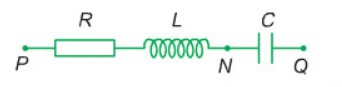
\includegraphics[scale=1.0]{../figs/VN12-PH-20-L-013-1-V2-01.jpg}
		\end{center}
		\begin{mcq}(4)
			\item $\dfrac{\sqrt{2}}{2}$.
			\item $\dfrac{\sqrt{3}}{2}$.
			\item $\dfrac{1}{2}$.
			\item $\dfrac{1}{4}$.
		\end{mcq}
	}
	{	\begin{center}
			\textbf{Hướng dẫn giải}
		\end{center}
		
		Điện áp hiệu dụng giữa hai đầu đoạn mạch PQ là:
		$$U_{\text{PQ}}=\sqrt{U_R^2+\left( U_L-U_C\right) ^2}=\sqrt{U_R^2+\left( U_L- 60\, \si{\volt}\right) ^2}=60\, \si{\volt}. $$
		
		Điện áp hiệu dụng giữa hai đầu đoạn mạch PN là:
		$$U_{\text{PN}}=\sqrt{U_R^2+U_L^2}=60\, \si{\volt}. $$
		
		Từ hai phương trình trên: $U_R= 30\sqrt{3}\, \text{V},U_L= 30\, \text{V}. $
		
		Hệ số công suất của mạch là
		$$\cos\varphi =\dfrac{U_R}{U}=\dfrac{\sqrt{3}}{2}. $$	
		
		\textbf{Đáp án: B}.
	}
	\viduii{3}{Một đoạn mạch xoay chiều gồm điện trở thuần $R$ mắc nối tiếp với cuộn dây. Biết điện áp hiệu dụng ở hai đầu cuộn dây là $\SI{45}{V}$, giữa hai đầu điện trở thuần là $\SI{30}{V}$, giữa hai đầu đoạn mạch là $\SI{60}{V}$. Hệ số công suất của cuộn dây là
		\begin{mcq}(4)
			\item 0,125.
			\item 0,15.
			\item 0,375.
			\item 0,25.
		\end{mcq}
	}
	{	\begin{center}
			\textbf{Hướng dẫn giải}
		\end{center}
		
		Ta có:
		$$U^2_r + U^2_L=45^2.$$
		
		Lại có:
		$$(30+ U_r)^2 + U^2_L =90^2 \Rightarrow U_r =\SI{11,25}{V}.$$
		
		Hệ số công suất của cuộn dây:
		$$\cos \varphi_\text{d} = \dfrac{r}{Z_\text{d}} = \dfrac{U_r}{U_\text{d}} =\text{0,25}.$$
		
		\textbf{Đáp án: D}.
	}
\end{dang}
\begin{dang}{Sử dụng được công thức tính công suất tiêu thụ trong mạch điện xoay chiều}
	\viduii{3}{Đặt điện áp $u = U_0\cos \left(\omega t + \dfrac{\pi}{3}\right)\ \text{V}$ vào hai đầu đoạn mạch gồm điện trở thuần, cuộn cảm thuần và tụ điện mắc nối tiếp. Biết cường độ dòng điện trong mạch có biểu thức $i = \sqrt 6 \left(\omega t + \dfrac{\pi}{6}\right)\ \text{A}$ và công suất tiêu thụ của đoạn mạch bằng 150 W. Giá trị $U_0$ bằng
		
		\begin{mcq}(4)
			\item 100 V.
			\item $100\sqrt 3$ V.
			\item 120 V.
			\item $100\sqrt 2$ V.
		\end{mcq}
	}
	{	\begin{center}
			\textbf{Hướng dẫn giải}
		\end{center}
		
		\begin{itemize}
			\item Cường độ dòng điện hiệu dụng
			\begin{equation*}
				I=\dfrac {I_0}{\sqrt 2}=\sqrt 3\ \text{A}.
			\end{equation*}
			\item Góc lệch pha giữa $u$ và $i$ trong mạch
			\begin{equation*}
				\varphi = \varphi_u-\varphi_i =\dfrac{\pi}{3}- \dfrac{\pi}{6}=\dfrac{\pi}{6}\ \text{rad}.
			\end{equation*}
			\item Công thức tính công suất tiêu thụ của mạch điện
			\begin{equation*}
				P=UI\cos \varphi.
			\end{equation*}
			\item Suy ra giá trị điện áp hiệu dụng
			\begin{equation*}
				U=\dfrac{P}{I\cos \varphi} = 120\ \text{V}.
			\end{equation*}
		\end{itemize}
		
		\textbf{Đáp án: C}.
	}
	\viduii{3}{Đặt một điện áp $u = 100\sqrt 2 \cos100\pi t\ \text{V}$, ($t$ đo bằng giây) vào hai đầu đoạn mạch gồm tụ $C$ nối tiếp với cuộn dây thì điện áp hiệu dụng trên tụ là $100\sqrt 3\ \text{V}$ và trên cuộn dây là 200 V. Điện trở thuần của cuộn dây là 50 $\Omega$. Công suất tiêu thụ điện của đoạn mạch là
		
		\begin{mcq} (4)
			\item 150 W.
			\item 100 W. 
			\item 120 W.
			\item 200 W.
		\end{mcq}
	}
	{	\begin{center}
			\textbf{Hướng dẫn giải}
		\end{center}
		
		\begin{itemize}
			\item Điện áp hai đầu cuộn dây 
			\begin{equation*}
				U^2_{\text{cd}}=U^2_r + U^2_L = 200^2.
			\end{equation*}
			\item Điện áp hiệu dụng hai đầu đoạn mạch 
			\begin{equation*}
				U=\dfrac{U_0}{\sqrt 2}=100\ \text{V}.
			\end{equation*}
			\item Điện áp hai đầu đoạn mạch
			\begin{equation*}
				U^2_{\text{cd}}=U^2_r + (U_L-U_C)^2 \Leftrightarrow U^2 =U^2_r + U^2_L - 2U_LU_C + U_C^2.
			\end{equation*}
			\item Thay các đại lượng đã cho vào biểu thức điện áp hai đầu đoạn mạch
			\begin{equation*}
				100^2 = 200^2  - 2 \cdot 100\sqrt 3 \cdot U_L + (100\sqrt 3)^2.	
			\end{equation*}
			\item Suy ra $U_L=100\sqrt 3\ \text{V}$ và $U_r= 100\ \text{V}$.
			\item Công suất tiêu thụ của đoạn mạch là 
			\begin{equation*}
				P=I^2r=\dfrac{U^2_r}{r} =200\ \text{W}
			\end{equation*}
		\end{itemize}
		
		\textbf{Đáp án: D}.
	}
	
	\viduii{3}{Cho đoạn mạch $RLC$, đặt vào đoạn mạch điện áp xoay chiều $u = U\sqrt 2 \cos 100\pi t\ \text{V}$. Khi $U =\SI{100}{V}$ thì cường độ dòng điện trong mạch trễ pha hơn điện áp là $\dfrac{\pi}{3}$ và công suất tỏa nhiệt của đoạn mạch là $\SI{50}{W}$. Khi $U =100\sqrt 3\ \text{V}$, để cường độ dòng điện hiệu dụng vẫn như cũ thì cần ghép nối tiếp với đoạn mạch trên điện trở $R_0$ có giá trị
		\begin{mcq}(4)
			\item $50\ \Omega$.
			\item $100\ \Omega$.
			\item $200\ \Omega$.
			\item $\text{73,2}\ \Omega$.
		\end{mcq}
	}
	{	\begin{center}
			\textbf{Hướng dẫn giải}
		\end{center}
		
		Xác định điện trở $R$:
		$$\calP = \dfrac{U^2}{R} \cos^2 \varphi \Rightarrow R = 50\ \Omega.$$
		
		Ta có:
		$$\tan \varphi = \dfrac{Z_L-Z_C}{R} = \tan \dfrac{\pi}{3}.$$
		
		$$\Rightarrow Z_L - Z_C = R\sqrt 3 = 50\sqrt 3\ \Omega.$$
		
		Ta lại có:
		$$I = I'$$
		$$\Rightarrow \dfrac{100\sqrt 3}{(R+R_0)^2 + (Z_L-Z_C)^2} = \dfrac{100}{\sqrt{R^2 + (Z_L-Z_C)^2}} $$
		$$\Rightarrow R_0 =100\ \Omega.$$
		
		\textbf{Đáp án: B}.
	}
	\viduii{3}{Đặt một điện áp $u = 100\sqrt 2\cos100 \pi t\ \text{V}$, ($t$ đo bằng giây) vào hai đầu đoạn mạch gồm tụ $C$ nối tiếp với cuộn dây thì điện áp hiệu dụng trên tụ là $100\sqrt 3\ \text{V}$ và trên cuộn dây là $\SI{200}{V}$. Điện trở thuần của cuộn dây là $50\ \Omega$ . Công suất tiêu thụ điện của đoạn mạch là
		\begin{mcq}(4)
			\item $\SI{150}{W}$.
			\item $\SI{100}{W}$.
			\item $\SI{120}{W}$.
			\item $\SI{200}{W}$.
		\end{mcq}
	}
	{	\begin{center}
			\textbf{Hướng dẫn giải}
		\end{center}
		
		Ta có:
		$$U^2_\text{d} =U^2_r + U^2_L = 200^2.$$
		$$U^2 =U^2_r +(U_L -U_C)^2 = U^2_r +U^2_L-2U_LU_C +U^2_C.$$
		
		Ta tìm được: 
		$$\Rightarrow U_L = 100\sqrt 3\ \text{V}; U_r =100\ \text{V}.$$
		
		Công suất tiêu thụ của đoạn mạch:
		$$\Rightarrow \calP =I^2r =\dfrac{U^2_r}{r} = \SI{200}{W}.$$
		
		\textbf{Đáp án: D}.
	}
\end{dang}